\chapter{Interférométrie}

\section{L'interféromètre de Fabry-Perot}
L’interféromètre de Fabry-Peret est composé de deux petits miroirs placés parallèlement l'un à 
l'autre et à distance contrôlée. Étudions ce dispositif à travers la lumière passant à travers 
deux miroirs\footnote{En réalité, la lumière passant à travers, il s'agit de \textit{semi-miroirs}.} 
parallèles.\\

	\begin{wrapfigure}[6]{l}{5cm}
	\vspace{-5mm}
	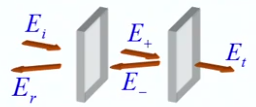
\includegraphics[scale=0.5]{ch4/image1.png}
	\captionof{figure}{ }
	\end{wrapfigure}
Le champ incident $E_i$ est partiellement transmis ($E_+$) et réfléchi ($E_r$). Il arrive sur 
le deuxième miroir où une partie est réfléchie dans la \textit{cavité optique} $E_-$ et une transmise 
par delà le second miroir, $E_t$. Le champ réfléchi $E_r$ comprend la contribution de l'ensemble 
du système comme nous le verrons plus tard. \\

	\begin{wrapfigure}[8]{r}{4.2cm}
	\vspace{-5mm}
	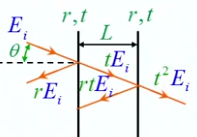
\includegraphics[scale=0.65]{ch4/image2.png}
	\captionof{figure}{ }
	\end{wrapfigure}
On peut s'intéresser aux \textit{réflexions multiples}. Représentons des miroirs comme 
des lames infiniment minces décrites par des coefficients de réflexion et transmission $r$ et $t$. 
On s'intéresse au cas du Fabry-Perot symétrique : les deux miroirs sont identiques, placés à une 
distance $L$. Un champ $E_i$ arrive sur le premier miroir à un angle d’incidence $\theta$ par 
rapport à la normale\footnote{Ce champ n'est pas "ponctuel" comme un laser mais bien une onde 
plane, comme le montre le schéma ci-dessus.}. Le coefficient de réflexion en amplitude $r$ nous 
donne le champ réfléchi : $rE_i$. De même, pour la transmission, $tE_i$ ect. pour le second miroir.\\

	\begin{wrapfigure}[8]{l}{4.2cm}
	\vspace{-5mm}
	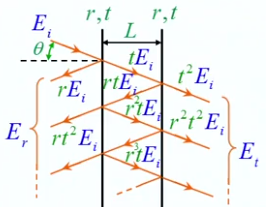
\includegraphics[scale=0.45]{ch4/image3.png}
	\captionof{figure}{ }
	\end{wrapfigure}
En suivant un raisonnement analogue pour le faisceau "dans" la cavité optique, il faut tenir compte 
les réflexions multiples qui contribuent aux champs totaux réfléchi $E_r$ et transmis $E_i$. On obtient 
alors une suite infinie de champs à considérer : principe de superposition. On pourrait étudier la 
convergence de la série mais nous allons quitter l'approche des réflexions multiples au profit d'une 
\textit{approche globale}.\\

	\begin{wrapfigure}[8]{r}{3cm}
	\vspace{-5mm}
	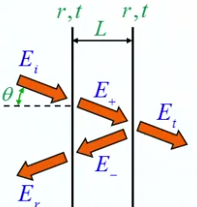
\includegraphics[scale=0.45]{ch4/image4.png}
	\captionof{figure}{ }
	\end{wrapfigure}
Considérons également un champ $E_i$ arrivant à un angle $\theta$. Par contre, dans la cavité, on 
considère un champ $E_+$ désignant l'ensemble des champs qui se propage dans le même sens que 
$E_i$ (dans $E_i$ se cache la somme $(t+rt+r^2t+\dots)E_i$). Ce $E_+$ engendre un champ $E_-$, soit 
la somme de toutes les ondes planes se déplaçant vers la gauche. Forcément, il y aura la 
transmission du champ $E_+$ donnant le champ transmis du Fabry-Perrot, $E_t$.\\

Pour connaître $E_t$, il faut passer par le calcul de $E_+$ et déduire le champ transmis par la 
transmission de $E_+$ : $E_t=tE_+$. De même, pour la réflexion : $E_r = rE_i+tE_-$. On ne fait 
rien d'autre que d'appliquer le principe de superposition.\\

	\begin{wrapfigure}[10]{l}{3.5cm}
	\vspace{-5mm}
	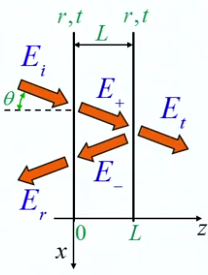
\includegraphics[scale=0.45]{ch4/image5.png}
	\captionof{figure}{ }
	\end{wrapfigure}
Faisons maintenant les choses de façon précises : on cherche à exprimer le champ transmis du 
Fabry-Perrot en fonction du champ incident. Bref, on cherche le "fonction de transfert". Pour 
commencer, il nous faut l'expression des champs eux-mêmes. Ce sont des ondes planes
\begin{equation}
\left\{\begin{array}{ll}
E_+ = \DS A_+e^{i\beta z}e^{i\rho x}\\
E_- = \DS A_-e^{-i\beta z}e^{i\rho x}
\end{array}\right.
\end{equation}
L'axe $x$ a été dirigé vers le bas afin que $\rho$, la projection du vecteur d'onde sur l'axe 
des $x$ soit positive, ayant choisi un rayon qui descend. Le $\beta$ représente ainsi la 
projection du vecteur d'onde sur l'axe $z$
\begin{equation}
\beta = k\cos\theta,\qquad \rho = k\sin\theta
\end{equation}
Pour l'onde réfléchie, on retrouve $-i\beta z$, l'onde se propageant vers les $z$ négatifs. 
Introduisons les conditions aux limites de cavité en tenant compte de l'endroit où cette 
condition est exprimée

\retenir{\ \textbf{Conditions aux limits de "cavité"}
\begin{enumerate}
\item $$E_t = tE_+(L) = tE_+(0)e^{i\beta L}$$
En effet, le champ en $L$ peut être exprimé avec celui en 0 (cf. système d'équation ci-dessus).
Les $e^{i\rho x}$ se simplifient : il ne faut pas en tenir compte (invariance sur l'axe $x$), 
nous ne tiendrons compte que des phases. 
\item $$E_+(0) = t_Ei+rE_-(0)$$
Il ne faut pas oublier la réflexion de $E_-$ en 0 qui vient "nourir" $E_+$.
\item $$E_-(0) = rE_+(L)e^{i\beta L} = rE_+(0)e^{2i\beta L}$$
Il s'agit de la réflexion de $E_+$ en $L$ mais en rajoutant toute la phase de propagation. 
S'il n'y a pas de signe négatif dans l'exponentielle, c'est parce que nous allons de $L$ en 
zéro.
\end{enumerate}}\ \\

Si l'on ne s'intéresse pas à $E_r$, nous avons trois inconnues : ces CL sont suffisantes. 
Considérons les combili de ces CL. En combinant (2) et (3)
\begin{equation}
E_+(0) = tE_i+r^2e^{2i\beta L}E_+(0)\quad\Leftrightarrow\quad E_+(0)[1-r^2e^{2i\beta L}] = tE_i
\end{equation}
L'inconnue étant éliminée, on trouve
\begin{equation}
E_+(0) = \dfrac{tE_i}{\DS 1-r^2e^{\DS 2i\beta L}}
\end{equation}
Il reste la CL (1) pour la transmission. En multipliant de part et d'autre par $te^{i\beta L}$
\begin{equation}
E_t = \dfrac{t^2E_i\ e^{i\beta L}}{\DS 1-r^2e^{2i\beta L}} = T_{FP}\times E_i
\end{equation}
On peut alors définir la fonction de transfert du Fabry-Perot. Tout le comportement du FP est 
exprimé dans cette fonction (pour la transmission).
\begin{equation}
T_{FP} = \dfrac{t^2\ e^{i\beta L}}{\DS 1-r^2e^{2i\beta L}}
\end{equation}
Intéressons-nous aux intensités
\begin{equation}
E_t = T_{FP}\times E_i\quad\Rightarrow\quad |E_t|^2 = |T_{FP}|^2 \times |E_i|^2
\end{equation}
où $|T_{FP}|^2 = \mathcal{T}$, la fonction de transmission en intensité.\\

Faisons une petite parenthèse : introduisons la fonction de transmission en intensité pour 
un miroire simple. Dans ce cas $E_t = tE_i$. Dès lors
\begin{equation}
|E_t|^2 = t^2|E_i|^2
\end{equation}
La \textit{transmission en intensité du miroir} vaut $T=t^2$. De même pour la \textit{réflectivité} 
$R=r^2$. Ceci permet d'introduire des concepts nouveaux. Partons de la conservation de l’énergie 
(supposé sans pertes, miroirs parfaits)
\begin{equation}
|E_t|^2+|E_r|^2=|E_i|^2
\end{equation}
Ceci donne lieu à une relation particulière entre $T$ et $R$
\begin{equation}
T|E_i|^2+R|E_i|^2 = |E_i|^2\qquad\Longrightarrow\qquad T+R=1
\end{equation}
C'est la conservation de l'énergie pour un miroir parfait. On peut ré-écrire la fonction de 
transmission compte-tenu de ceci :
\begin{equation}
T_{FP} = \dfrac{(1-R)e^{i\beta L}}{1-Re^{2i\beta L}}
\end{equation}
Fin de la parenthèse, revenons à nos moutons : exprimons $\mathcal{F}$ 
\begin{equation}
\mathcal{F} = \dfrac{(1-R)^2}{|1-R[\cos(2\beta L)+i\sin(2\beta L)]|^2}
\end{equation}
En calculant le dénominateur
\begin{equation}
\mathcal{F} = \dfrac{(1-R)^2}{[1-R\cos(2\beta L)]^2+R^2\sin^2(2\beta L)} = \dfrac{(1-R)^2}{
1-2R\cos(2\beta L)+R^2\cos^2(2\beta L)+R^2\sin^2(2\beta L)}
\end{equation}
Avec l'identité fondamentale
\begin{equation}
\mathcal{T} = \dfrac{(1-R)^2}{1-2R\cos(2\beta L)+R^2}
\end{equation}
Sachant que $\cos(2\theta) = 1-2\sin^2(\theta)$
\begin{equation}
\mathcal{T} = \dfrac{(1-R)^2}{\underbrace{1-2R+R^2}_{(1-R)^2}+4R\sin^2(\beta L)} = 
\dfrac{1}{1+\dfrac{4R\sin^2(\beta L)}{(1-R)^2}}
\end{equation}
En posant $\DS F=\frac{4R}{(1-R)^2}$, la \textit{finesse} du FB.


\retenir{\ \textbf{Fonction d'Airy}
\begin{equation}
\mathcal{T} = \dfrac{1}{1+F\sin^2(\beta L)}
\end{equation}
Ceci caractérise le FB en fonction de l'intensité lumineuse.}\ \\

Rappelons 
\begin{equation}
F = \dfrac{4R}{(1-R)^2},\qquad \beta = k_0\cos\theta
\end{equation}
Choisissons $R=0.17$ tel que $F = 1$. Nous pouvons alors représenter $\mathcal{T}$ 
graphiquement. Il s'agit d'une fonction périodique de fonction $\pi$, le sinus étant 
au carré. Aux multiples de $\pi$, on récupère une transmission unitaire. Entre les pics, on 
obtient un minimum pour $(2n+1)\frac{\pi}{2}$.  

\begin{center}
	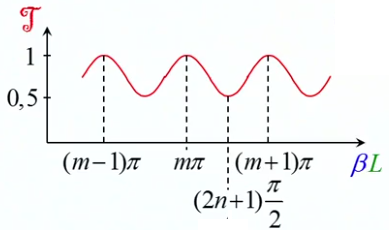
\includegraphics[scale=0.45]{ch4/image6.png}
	\captionof{figure}{ }
\end{center}

On peut maintenant s'intéresser à la réflexion. En définissant la fonction de transmission 
en intensité du FB 
\begin{equation}
|E_r|^2 = \mathcal{R}\times|E_i|^2
\end{equation}
Pas besoin de chercher de 12 à 14h : $\mathcal{R}+\mathcal{T}=1$, les miroirs étant sans 
pertes. 

\begin{center}
	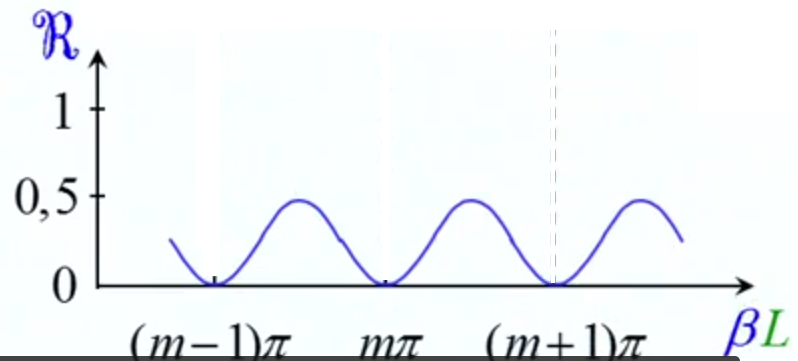
\includegraphics[scale=0.25]{ch4/image7.png}
	\captionof{figure}{ }
\end{center}

Ceci montre que lorsque $\beta L = n\pi$, nous aurons un zéro. Ce résultat est totalement 
indépendant de $R$ et $F$. Dès lors, en prenant un miroir où $R=99.99\%$ de réflexion, 
toute la lumière qui arrive passe au travers. C'est une belle surprise. 






































